% \iffalse
\let\negmedspace\undefined
\let\negthickspace\undefined
\documentclass[journal,12pt,twocolumn]{IEEEtran}
\usepackage{cite}
\usepackage{amsmath,amssymb,amsfonts,amsthm}
\usepackage{algorithmic}
\usepackage{graphicx}
\usepackage{textcomp}
\usepackage{xcolor}
\usepackage{txfonts}
\usepackage{listings}
\usepackage{enumitem}
\usepackage{mathtools}
\usepackage{gensymb}
\usepackage{comment}
\usepackage[breaklinks=true]{hyperref}
\usepackage{tkz-euclide} 
\usepackage{listings}
\usepackage{gvv}                                        
\def\inputGnumericTable{}                                 
\usepackage[latin1]{inputenc}                                
\usepackage{color}                                            
\usepackage{array}                                            
\usepackage{longtable}                                       
\usepackage{calc}                                             
\usepackage{multirow}                                         
\usepackage{hhline}                                           
\usepackage{ifthen}                                           
\usepackage{lscape}
\usepackage[center]{caption} % center the captions to figure

\newtheorem{theorem}{Theorem}[section]
\newtheorem{problem}{Problem}
\newtheorem{proposition}{Proposition}[section]
\newtheorem{lemma}{Lemma}[section]
\newtheorem{corollary}[theorem]{Corollary}
\newtheorem{example}{Example}[section]
\newtheorem{definition}[problem]{Definition}
\newcommand{\BEQA}{\begin{eqnarray}}
\newcommand{\EEQA}{\end{eqnarray}}
\newcommand{\define}{\stackrel{\triangle}{=}}
\theoremstyle{remark}
\newtheorem{rem}{Remark}
\begin{document}

\newcolumntype{M}[1]{>{\centering\arraybackslash}m{#1}}
\newcolumntype{N}{@{}m{0pt}@{}}

\bibliographystyle{IEEEtran}
\vspace{3cm}

\title{NCERT 11.9.3 5Q} 
\author{ee23btech11223 - Soham Prabhakar More% <-this % stops a space
}
\maketitle
\newpage
\bigskip

\renewcommand{\thefigure}{\theenumi}
\renewcommand{\thetable}{\theenumi}

\bibliographystyle{IEEEtran}

\textbf{Question:}\\
Which term of the following sequences:\\
(a) 2,$2\sqrt{2}$,4\dots is 128
\quad(b) $\sqrt{3}$,3,$3\sqrt{3}$\dots is 729\\
(c) $\frac{1}{3}$,$\frac{1}{9}$,$\frac{1}{27}$\dots is $\frac{1}{19683}$

\textbf{Answer:} For a general GP series and $k > 0$,
\begin{align}
    x\brak{k} &= x\brak{0}r^k \\
    \therefore k &= \log_r{\frac{x\brak{k}}{x\brak{0}}} \label{eq:gsoln}
\end{align}
And the Z-transform $X\brak{z}$:
\begin{align}
    X\brak{z} &= \frac{x\brak{0}}{1 - rz^{-1}} \quad {\abs{z} > \abs{r}} \label{eq:zresult}
\end{align}

\begin{enumerate}[label=(\alph*)]
\item By \tabref{Table:1}, \eqref{eq:gsoln} and \tabref{Table:1}: % prob:a
\begin{align}
    x_1\brak{n} &= x_1\brak{0} r_1^nu\brak{n} \\
    k_1 &= \log_{r_1}{\frac{128}{x_1\brak{0}}} \\
    \therefore k_1 &= 12 \\
	X_1\brak{z} &= \frac{2}{1 - \sqrt{2}z^{-1}} \quad \abs{z} > \sqrt{2}
\end{align}

\begin{figure}[h!]
    \renewcommand\thefigure{1}
    \centering
    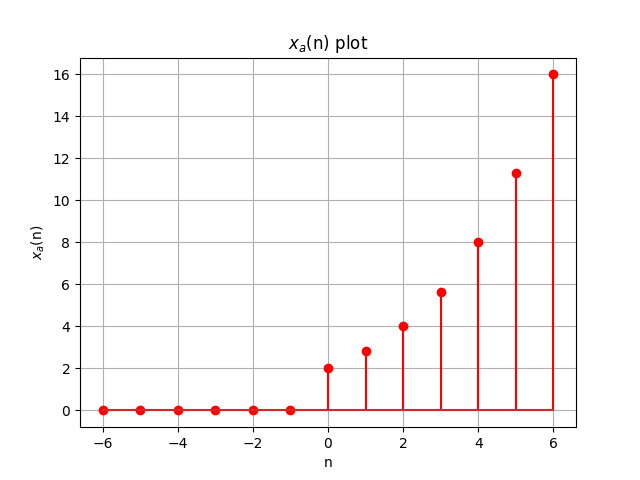
\includegraphics[width=\columnwidth]{figs/a.png}
    \caption[short]{Plot of $x_1$\brak{n} vs n. See \tabref{Table:1}}
    \label{fig:img1}
\end{figure}



\item By \eqref{eq:gsoln}, \eqref{eq:zresult} and \tabref{Table:1}: % prob:b
\begin{align}
    x_2\brak{n} &= x_2\brak{0} r_2^nu\brak{n} \\
    k_2 &= \log_{r_2}{\frac{729}{x_2\brak{0}}} \\
    \therefore k_2 &= 11 \\
    X_2\brak{z} &= \frac{\sqrt{3}}{1 - \sqrt{3}z^{-1}} \quad \abs{z} > \sqrt{3} 
\end{align}

\begin{figure}[h!]
    \renewcommand\thefigure{2}
    \centering
    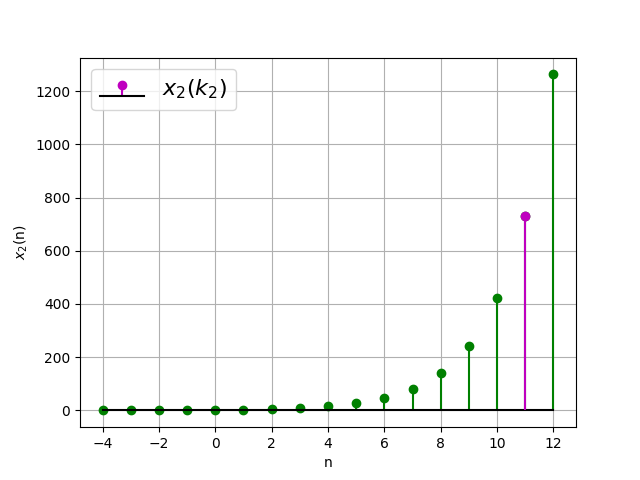
\includegraphics[width=\columnwidth]{figs/b.png}
    \caption[short]{Plot of $x_2$\brak{n} vs n. See \tabref{Table:1}}
    \label{fig:img2}
\end{figure}

\item By \eqref{eq:gsoln}, \eqref{eq:zresult} and \tabref{Table:1}: % prob:c
\begin{align}
    x_3\brak{n} &= x_3\brak{0} r_3^nu\brak{n} \\
    k_3 &= \log_{r_3}{\frac{1}{19683 x_3\brak{0}}} \\
    \therefore k_3 &= 8 \\
    X_3\brak{z} &= \frac{1}{3 - z^{-1}} \quad \abs{z} > \frac{1}{3}
\end{align}

\begin{figure}[h!]
    \renewcommand\thefigure{3}
    \centering
    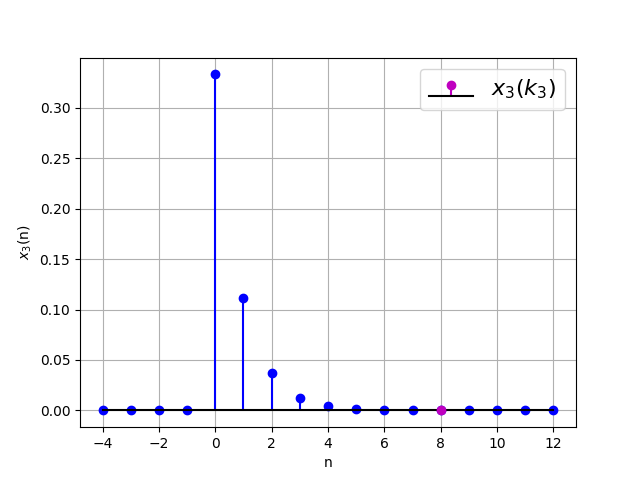
\includegraphics[width=\columnwidth]{figs/c.png}
    \caption[short]{Plot of $x_3$\brak{n} vs n. See \tabref{Table:1}}
    \label{fig:img3}
\end{figure}

\begin{table}[ht]
\renewcommand\thetable{1}
\begin{tabular}{|c|c|}
    \hline 
    \textbf{Parameter}&\textbf{Description} \\
    \hline
    $F\brak{s}$ & Laplace transform of $\delta\brak{t - a}$ \\
    \hline
    $G\brak{f}$ & Fourier transform of $\delta\brak{t - a}$ \\
    \hline
    $w_T\brak{t}$ & Delta Comb, $\sum_{k = -\infty}^{\infty}\delta\brak{t - kT}$ \\
    \hline
    $W_T\brak{t}$ & Fourier transform of $w_T\brak{t}$ \\
    \hline
\end{tabular}

\caption{Table of parameters}
\label{Table:2022.ME.3.1}


\end{table}

\end{enumerate}

\end{document}

